\section{Models of Extra-functional Properties}\label{sec_extrafunc}
In this section, we discuss the timing, application reliability, and power consumption models used throughout the paper.

\subsection{Power Consumption Model}
Power consumption refers to the energy usage of electronic components in an integrated circuit, e.g., processor, memory, I/O devices, etc., per time unit. Depending on the nature of the integrated circuit and intended use, there exist low-level and high-level models of power and energy consumption estimation techniques. The low-level models, for instance in CMOS-based integrated circuits estimate power consumption via the power consumption of flip-flops and combinatorial gates \cite{Najm1994ACircuits}\cite{Najm1995PowerCircuits}, and they are frequently used in the design of power-efficient electronic circuits designs. The high-level models apply dynamic profiling of computer components, e.g., CPU, memory, I/O devices, etc., to estimate power consumption of the computer system, and they are primarily used in energy management techniques, e.g., in dynamic Voltage and Frequency Scaling (DVFS) \cite{Contreras2005PowerEvents}.

However, the previously mentioned power estimation techniques have limitations especially for applications in the early stages of system design. Their limitations are as follows: i) the lack of complete and accurate information of electrical specification of integrated circuits makes the use of low-level power estimation methods difficult, and ii) the dynamic profiling of high-level techniques requires runtime mechanisms, such as performance counter monitor, which is not applicable in our case. Instead, in this work, we employ a different approach that is based on processor load (or \textit{Processor Utilization}) to estimate the average power consumption of a computational node. Specifically, we use the linear polynomial model proposed by Fan et al. \cite{Fan2007PowerComputer}, which is shown in (\ref{eqn_powerconsumption}). The mode states that the power consumption of a node is directly proportional to its load, and is inductively formulated from experimental results:
\begin{equation}
\label{eqn_powerconsumption}
f_p(u)=P_{idle} + (P_{busy}-P_{idle})*u,
\end{equation}

where $u$ is the utilization (or load) of a computation node, $p_{idle}$ and $p_{busy}$, respectively, refer to the power consumption of a node measured at minimum and maximum processor loads. Such measurements can be obtained by running performance benchmark suits, e.g., MiBench \cite{Guthaus2001MiBench:Suite}, AutoBench \cite{EMBC2018AutoBenchProcessors}, etc.
\begin{figure*}[h!]
    \centering
    \begin{subfigure}[b]{0.25\textwidth}
    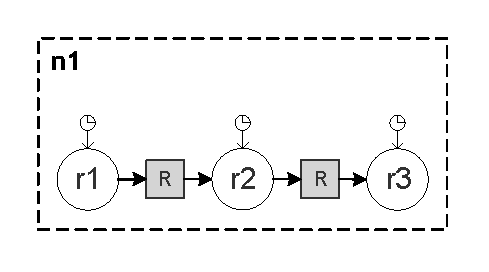
\includegraphics[trim=0 0 0 0,clip,width=\textwidth]{datachain_singlenode}
    \caption{Deployment on a Single Node.}
    \label{fig_datachainsingle}
    \end{subfigure}
    ~ %\quad, \qquad, \hfill 
    \begin{subfigure}[b]{0.365\textwidth}
    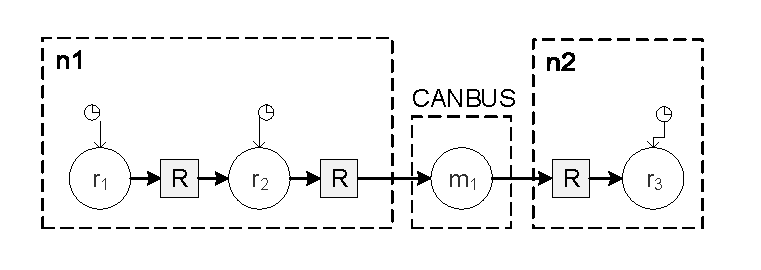
\includegraphics[trim=0 0 0 0,clip,width=\textwidth]{datachain_multinode}
    \caption{Deployment on Multiple Nodes.}
    \label{fig_datachainmulti}
    \end{subfigure}
   ~\vspace{-0.2cm}
    \begin{subfigure}[b]{0.35\textwidth}
    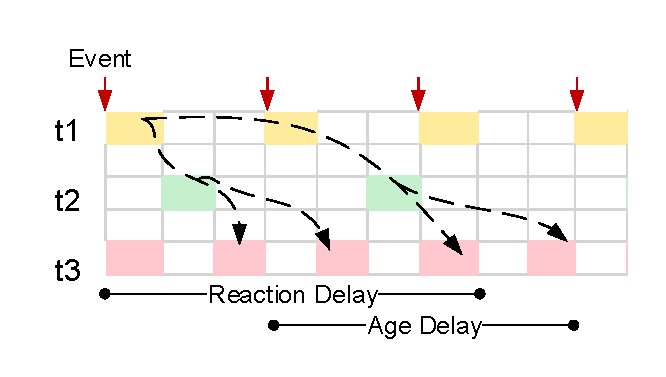
\includegraphics[width=\textwidth]{timedpath}
    \caption{Timed Paths of Age and Reaction Delays.}
    \label{fig_timedpath}
    \end{subfigure}
    \caption{Cause-effect Chain with Three Activation Patterns.}
    \label{fig:datachain}
\end{figure*}

\subsection{Software Application Reliability}
\textit{Application reliability} $R_a$ refers to the probability that a software application functions correctly by the time $t$, or within the time interval $[0, t]$ \cite{Goel1985SoftwareApplicability}. We assume that  applications are free from design errors and, therefore, an application failure can be caused only by failures from the computational nodes in which the application is deployed. The failure rate of a node over time is represented by $\lambda(t)$, and the reliability of a node is represented by the exponential density function over constant failure rate $\lambda e^{-\lambda t}$, where $\lambda=\lambda(t)$.

In a system without replication, the failure of any arbitrary node that hosts the software application renders the whole application faulty. Reliability calculation is then straightforward, using a series-parallel model: $R_a = \prod_{m\in M}r_m$.  However, with the introduction of replication, to enable fault tolerance, the reliability calculation is not straightforward due to the replicas of the same software component allocated to different nodes that result in functional interdependencies between nodes. A software application functions \textit{ correctly} if each software component is executed at least by one non-faulty node, and will be \textit{faulty} otherwise (i.e., if there are one or more software components that are allocated only to faulty nodes and thus these components cannot be executed correctly).

To calculate the reliability in such cases, we use state enumeration, which is one of the reliability-preserving methods that are used to compute the reliability of a system with dependent components (or subsystems) \cite{Lucet1999ExactReliability}. The state enumeration method allows the exploration of all possible states of a system in the probability space $P\!S$. Our goal is to differentiate between the states in which the application functions, denoted by \textit{Functions(s)}, and the states in which the application fails, denoted by \textit{Fails(s)}. The application reliability $R_a$ is then calculated as follows:
\begin{equation}
\label{eqn_appreliability}
R_a=\sum_{s\in PS|Functions(s)}p_s=1-\sum_{s\in PS|Fails(s)}p_s
\end{equation}

To obtain $p_s$, that means the probability that the application is in state $s\in PS$, we define the Boolean variable $z_m \in \{0,1\}$ to indicate whether a node $m \in M$ is either faulty, $z_m = 0$, or not, $z_m = 1$. Then, the probability is calculated using (´\ref{eqn_stateprobability}).
\begin{align}
\label{eqn_stateprobability}
p_s=\prod_{m\in M}((z_m*r_m) + (1-z_m)*(1-r_m)),
\end{align}
where $r_m$ and $1-r_m$ are a computation node's reliability and probability of failure, respectively.

\subsection{The Timing Model}
The software application can be considered as a set of cause-effect chains, which are directed paths in the application graph, e.g.,  activation of a cruise control system by pressing a rotary-wheel on the dashboard, slowing down of a car by pressing the brake pedal, etc. Each cause-effect chain is annotated with an end-to-end timing requirement that specifies the maximum time between a stimulus and the corresponding response of a chain. A cause-effect chain can be hosted on a single node or multiple nodes as illustrated in Figure \ref{fig_datachainsingle} and Figure \ref{fig_datachainmulti}, respectively. Moreover, it can be activated by a single activation pattern, or multiple activation patterns (multirate).

The calculation of data-propagation delays in multirate software applications is not trivial due to the oversampling and undersampling effects, caused by the different activation patterns. Consequently, there are different delay semantics, which differ depending on the timed paths through which the data is propagated from the input to the output of the chains~\cite{mubeen2013support}. In this work, we focus on the \textit{age} and \textit{reaction} delays, which are the most widely used delay semantics in the automotive embedded systems. The two delays in a cause-effect chain that is distributed over two nodes  are demonstrated in Figure~\ref{fig_timedpath}. The tasks t1 and t2 execute on one node, whereas task t3 executes on the second node. Note that t2 communicates with t3 via a network message, that is not shown in the figure for simplicity. The red inverted arrows in Figure~\ref{fig_timedpath} represent the arrival of events at the input of the chain, whereas the dashed-curve arrows represent the timed paths through which the data propagates from the input to the output of the chain. The age delay is the time elapsed between a stimulus and its corresponding latest non-overwritten response, i.e., between the $2^{nd}$ instance of t1 and the $5^{th}$ instance of t3. This delay is frequently used in the control systems applications where freshness of data is paramount. For example, the torque applied to turn the wheels must correspond to the position of the steering wheel and must be time bound. The reaction delay is the earliest time the system takes to respond to a stimulus that ``just missed" the read access at the input of the chain. Assume that an event occurs just after the start of execution of the $1^{st}$ instance of t1. The data corresponding to this event is not read by the current instance of t1. In fact, the data will be read by the $2^{nd}$ instance of t1. The earliest effect of this event at the output of the chain will appear at the $4^{th}$ instance of t3, which represents the reaction delay. This delay is useful in body-electronics domain where first reaction to events is important, e.g., in the button-to-reaction applications. We refer the reader to \cite{mubeen2013support} for the formal semantics of the two delays used in this paper.


\subsection{Running Example}
The example employs an AUTOSAR system, which consists of a software application model and a hardware platform model, as well as functional and extra-functional requirements such as timing and reliability of the software application. The software application is modeled as a digraph of runnables, which is shown in Figure \ref{fig_application}. It consist of 50 runnables, 35 cause-effect chains (or paths), with their activation patterns and timing specifications shown in Table \ref{tbl_requirements}. The timing specifications of the runnables as well as the software components from which the runnables are instantiated are shown in Table \ref{tbl_comps_config}. The hardware platform model consists of three computation nodes, with specifications shown in Table \ref{tbl_nodes_specification}.
\begin{figure}[t!]
\centering
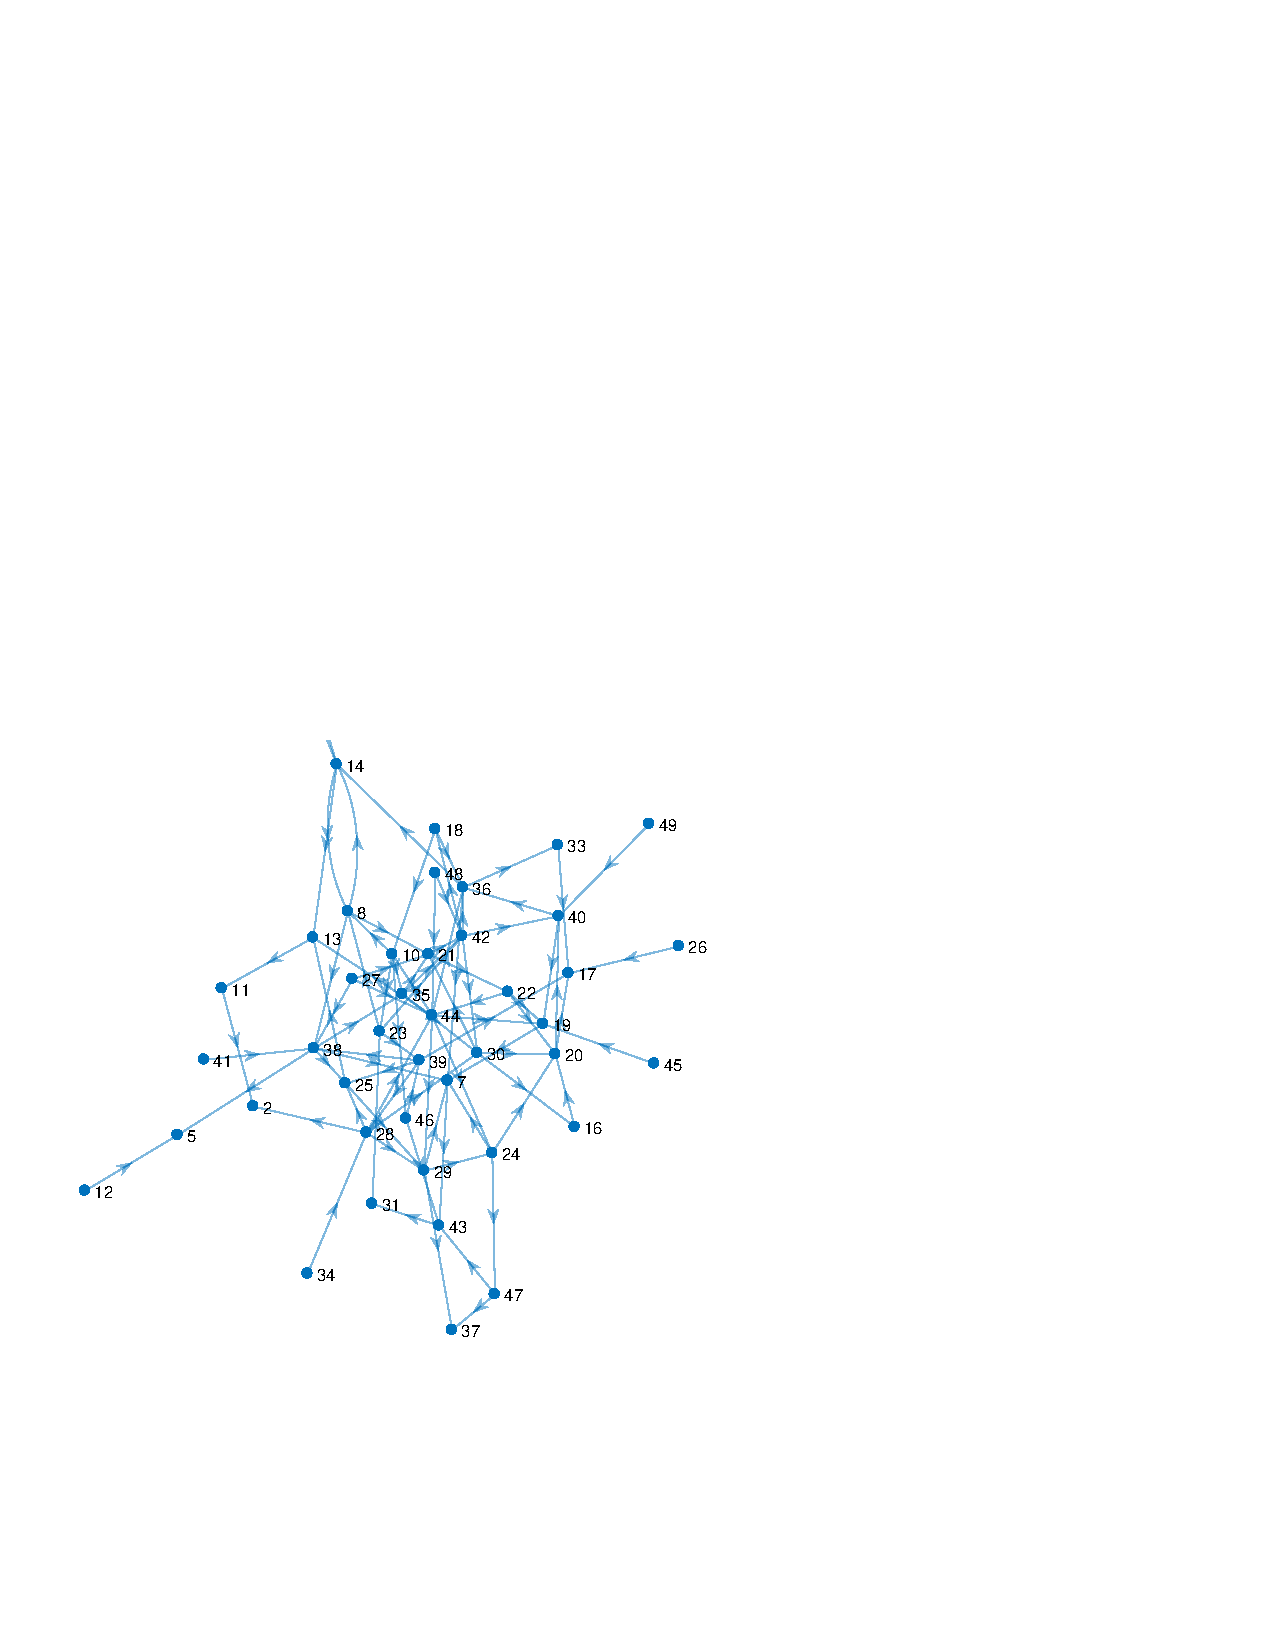
\includegraphics[width=0.8\linewidth]{dag}
\caption{A Directed Acyclic Graph of the Running AUTOSAR Software Application, Runnables = 50, Paths = 35, Activation Patterns shown in Table \ref{tbl_requirements}.}
\label{fig_application}
\end{figure}
\begin{center}
\small
\begin{minipage}{.5\textwidth}%
\centering
\begin{tabular}{@{}p{0.25cm}lll@{}}
\toprule
C& $r_i$ & $(e_{r_im_1}, e_{r_im_2}, e_{r_im_3})$ & $period$\\ \midrule
\multirow{4}{4em}{c1} 
&$r_1$ & (0.030, 0.060, 0.090) & 1\\
&$r_2$ & (0.041, 0.081, 0.122) & 2\\
&$r_3$ & (0.083, 0.167, 0.250)  & 5\\ 
&$r_4$ & (0.310, 0.620, 0.930) & 10 \\[0.3em]
\multirow{2}{4em}{c2} 
&$r_1$ & (0.310, 0.620, 0.930) & 10\\
&$r_2$ & (0.310, 0.620, 0.930) & 10\\
&$r_3$ & (0.310, 0.620, 0.930)  & 10\\ 
&$r_4$ & (0.310, 0.620, 0.930) & 10 \\[0.3em]
\multirow{2}{4em}{c3} 
&$r_1$ & (0.310, 0.620, 0.930) & 10\\
&$r_2$ & (0.291, 0.583, 0.874)) & 10\\
&$r_3$ & (0.291, 0.583, 0.874)  & 20\\ 
&$r_4$ & (0.291, 0.583, 0.874) & 20 \\[0.3em]
\multirow{2}{4em}{c4} 
&$r_1$ & (0.291, 0.583, 0.874) & 20\\
&$r_2$ & (0.291, 0.583, 0.874)) & 10\\
&$r_3$ & (0.291, 0.583, 0.874)  & 20\\ 
&$r_4$ & (0.093, 0.186, 0.279) & 50 \\[0.3em]
\multirow{2}{4em}{c5} 
&$r_1$ & (0.420, 0.841, 1.261) & 100\\
&$r_2$ & (0.420, 0.841, 1.261)) & 100\\
&$r_3$ & (0.420, 0.841, 1.261)  & 100\\ 
&$r_4$ & (0.420, 0.841, 1.261) & 100 \\[0.3em]
\bottomrule
\end{tabular}
\captionof{table}{Specification of Components.}
\label{tbl_comps_config}
\end{minipage}~
\begin{minipage}{.45\textwidth}
\begin{center}
    \begin{tabular}{@{}lll@{}}
    \toprule
    Activation, $AP$ & Share & Time, ms \\ \midrule
    $\tau_1$ & 0.5  & 50\\
    $\tau_1\rightarrow\tau_2$ & 0.2  & 100\\
    $\tau_1\rightarrow\tau_2\rightarrow\tau_3$ & 0.2  & 200\\
    $\tau_1\rightarrow\tau_2\rightarrow\tau_3\rightarrow\tau_4$ & 0.1  & 400\\
    \bottomrule
    \end{tabular}
    \captionof{table}{Activation Patters of Cause-effect Chains, their Share and End-to-end Timing Requirements.}
    \label{tbl_requirements}
\end{center}
\begin{center}
    \begin{tabular}{@{}llll@{}}
    \toprule
    M  & $P_{idle}$& $P_{busy}$& $\lambda$ \\ \midrule
    $m_1$ & 50.0& 140.0 &1.0E-3  \\
    $m_2$ & 10.0& 100.0 &1.0E-4  \\
    $m_3$ & 10.0& 140.0 &1 .0E-5 \\ \bottomrule
    \end{tabular}
    \captionof{table}{Computation Nodes Specification.}
    \label{tbl_nodes_specification}
\end{center}
\end{minipage}
\end{center}

In the next subsequent subsections, we propose an ILP mode and a PSO algorithm that encodes the software allocation problem. Furthermore, we elaborate concepts of the proposed solutions via the running example.
